


\subsection{Electrical design}

The electrical design of our payload relies on the use of custom-made PCBs due to the limited space available in its interior. We have developed custom PCBs designed using Autodesk's EAGLE software to ensure that all the necessary components fit properly. 

Using custom PCBs provides several advantages for the CanSat project. Firstly, it allows for a better fit of all the components in the limited space available. This can increase the overall efficiency of the payload by reducing the size and weight while still accommodating all the necessary components. Secondly, custom PCBs can also help to reduce the risk of damage to the components during the launch and landing phases of the mission. By integrating the components into the PCB design, they are better protected from shocks and vibrations. Finally, designing custom PCBs allows for greater flexibility and customization in the CanSat's design, making it possible to optimize its performance and tailor it to specific mission requirements.

\subsubsection{Electrical Interface}
The electrical interface of the CanSat is designed to ensure a robust and reliable connection between its various electronic components. The microcontroller, an RP2040 / ESP32, serves as the central hub for the electrical interface, supplying power and data connectivity to the array of sensors, transmitters, and other components on the Sensor and Communications Boards.

\begin{figure}[htbp]
\centering
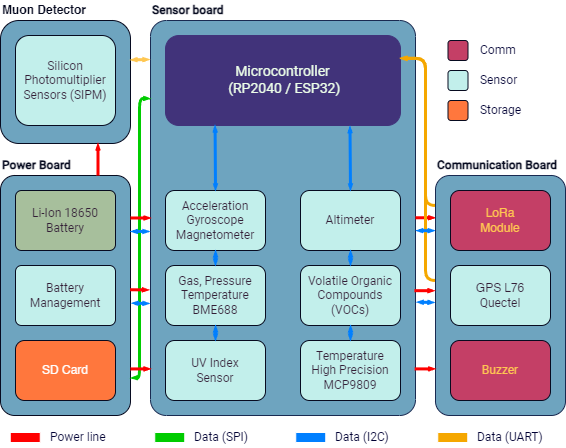
\includegraphics[width=0.7\linewidth]{images/img_module_diagram_new.png}
\caption{\small{The Cansat block diagram with power and data lines.}}
\label{figmodule_diagrame}
\end{figure}

The compact form factor of the payload's mainboard is tailored to accommodate the RP2040 / ESP32 microcontroller. This component is chosen for its adequate computing power and integrated wireless communication capabilities, vital for the mission. To ensure compatibility and flexibility, multiple connection types are established between the microcontroller and other components, including UART, I2C, SPI, and other necessary digital inputs and outputs.

The environmental sensors, measuring atmospheric pressure, temperature, humidity, and UV index, are integrated onto the same PCB as the microcontroller to streamline data line connectivity, utilizing I2C connections for efficient communication. The Silicon Photomultiplier Sensors (SiPM) for muon detection communicate via the SPI/UART protocol. All data collected by the sensors are logged onto an onboard SD card and transmitted to the base station.


\begin{table}[htbp]
\centering
\arrayrulecolor{DeepSkyBlue4}
\begin{tabularx}{0.95\textwidth}{>{\raggedright\arraybackslash}p{3.5cm}c>{\raggedright\arraybackslash}X>{\raggedright\arraybackslash}p{5.5cm}}
\hline
\rowcolor{DeepSkyBlue4}
\textbf{\color{white!50}{Component}} & \textbf{\color{white!50}{Voltage}} & \textbf{\color{white!50}\textbf{Protocol}} & \textbf{\color{white!50}\textbf{Other Information}} \\ \hline
\rowcolors{2}{red}{}
ESP32-S3-Wroom or Raspberry Pi 20400& \SI{3.3}{\volt} & I2C, I2S, SPI, PWM, UART, USB & {Dual-core $\mu$Processor}\\ %\hline
% \rowcolor{LightCyan1!50}ESP32 Cam Board & \SI{3.3}{\volt} & I2C, SPI, PWM, UART & {Dual-core $\mu$Processor}\\ %$\hline
% Arduino Nano 33 BLE Sense & \SI{3.3}{\volt} & I2C, SPI, PWM, UART & {$\mu$Processor}\\ %\hline
\rowcolor{LightCyan1!50}LPS25H & \SI{3.3}{\volt} & I2C & Altimeter\\ %\hline
MPU-9250 & \SI{3.3}{\volt} & I2C & MEMS Module, 6-Axis Gyroscope,\/ Accelerometer,\/ Magnetometer\\ %\hline
\rowcolor{LightCyan1!50}BME688 & \SI{3.3}{\volt} & I2C & Air Quality Sensor, Humidity, Pressure \& Temperature Sensor\\ %\hline
MCP9808 & \SI{3.3}{\volt} & I2C & Temperature Sensor\\ %\hline
\rowcolor{LightCyan1!50}VEML6075 & \SI{3.3}{\volt} & I2C & Ambient Light Sensor\\ %\hline
Quectel L76 & \SI{3.3}{\volt} & UART, I2C & GNSS / GPS Module\\ %\hline
\rowcolor{LightCyan1!50}micro SD & \SI{3.3}{\volt} & SPI & Memory Card Connector\\ %\hline
LoRa Module& \SI{3.3}{\volt} & UART & Lora Modulation, \SI{868}{\mega\hertz} \\ %\hline
\rowcolor{LightCyan1!50}Power Switching Regulators & \SI{3.3}{\volt} & & High Efficiency Buck-Boost Converter  \\ %\hline
Low-dropout regulator& \SI{3.3}{\volt} & & Voltage regulator, \SI{868}{\mega\hertz} \\ %\hline
\rowcolor{LightCyan1!50}Muon detector & \SI{25}{\volt} & & Silicon Photomultiplier Sensor (SIPM)  \\ %\hline
\end{tabularx}
\caption{\small{Electronics Component Information}}
\end{table}

The power system is centered around a Li-Ion battery, managed by a battery management system to ensure optimal performance and safety. The microcontroller and low-power sensors are energized by a 3.3 Volt line from the Power Board. In contrast, the muon detector module, requiring a different voltage line, will be adequately supported by the power system design. The battery pack's voltage range, from 3.6V to 4.2V, is compatible with the system requirements. Voltage regulation is achieved through the use of buck-boost converters and low-dropout regulators, ensuring that all components receive the correct voltage. These converters are rated to deliver up to 2A of continuous current, enough to power the entire system without risk of overloading any component.

The operational time of the Payload (for the single battery case) can be estimated with the given formula:

\begin{equation*}
\text{Time} = \frac{\text{Battery capacity} * \text{Voltage}}{\text{Power consumption}}=\frac{\SI{3400}{\milli\ampere} * \SI{4.2}{\volt}}{\SI{4.63}{\watt}} = \SI{3}{\hour} 
 05\text{min}
\end{equation*}

The duration of 3 hour is applicable when the payload's electronics operate at full capacity. With a dual battery system, this operational time significantly extends to well over 6 hours.

\begin{table}[htbp]
\centering
\arrayrulecolor{DeepSkyBlue4}
\begin{tabular}{>{\raggedright\arraybackslash}p{5cm}c>{\raggedleft\arraybackslash}p{2cm}
>{\raggedleft\arraybackslash}p{3cm}>{\centering\arraybackslash}p{2cm}>{\centering\arraybackslash}p{2cm}}
\hline
\rowcolor{DeepSkyBlue4}
\textbf{\color{white!50}{Component}} & \textbf{\color{white!50}{Voltage}} & \textbf{\color{white!50}\textbf{Current}} & \textbf{\color{white!50}\textbf{Power}} & \textbf{\color{white!50}\textbf{Mass}} \\ \hline
\rowcolors{2}{red}{}
ESP32 / RP2040 & \SI{3.3}{\volt} & \SI{40}-\SI{240}{\milli\ampere} & \SI{0.132}-\SI{0.792}{\watt} & \SI{2.15}{\gram}  \\
\rowcolor{LightCyan1!50}LPS25H & \SI{3.3}{\volt} & \SI{6}{\milli\ampere} & \SI{0.0198}{\watt} & \SI{0.8}{\gram}  \\
MPU-9250 & \SI{3.3}{\volt} & \SI{3.9}{\milli\ampere} &  \SI{0.01287}{\watt} &\SI{2.1}{\gram} \\
\rowcolor{LightCyan1!50}BME688 & \SI{3.3}{\volt} & \SI{3.9}{\milli\ampere} & \SI{0.01287}{\watt} & \SI{1.7}{\gram}  \\
MCP9808 & \SI{3.3}{\volt} & \SI{0.2}{\milli\ampere} &  \SI{0.00066}{\watt} &\SI{0.9}{\gram} \\
\rowcolor{LightCyan1!50}VEML76075 & \SI{3.3}{\volt} & \SI{0.12}{\milli\ampere} &  \SI{0.0004}{\watt} &\SI{0.8}{\gram}  \\
Quectel L76 (GPS) & \SI{3.3}{\volt} &  \SI{25}{\milli\ampere} &  \SI{0.0825}{\watt} & \SI{0.5}{\gram} \\
\rowcolor{LightCyan1!50}micro SD & \SI{3.3}{\volt} & \SI{0.2}{\milli\ampere} &  \SI{0.00066}{\watt} &\SI{1.6}{\gram} \\
LoRa Module & \SI{3.3}{\volt} & \SI{40}{\milli\ampere} &  \SI{0.132}{\watt} &\SI{4.15}{\gram} \\
\rowcolor{LightCyan1!50}Power Switching Regulators & \SI{3.3}{\volt} &\SI{800}{\milli\ampere}&  \SI{2.64}{\watt} &\SI{0.7}{\gram}\\
Low-dropout regulator & \SI{3.3}{\volt} &\SI{100}{\milli\ampere}&  \SI{0.3}{\watt} &\SI{0.6}{\gram}  \\
\rowcolor{LightCyan1!50}Muon detector & \SI{25}{\volt} & \SI{0.02}{\milli\ampere} & \SI{0.5}{\watt} &\SI{7}{\gram} \\ 
Buzzer & \SI{3.3}{\volt} &\SI{30}{\milli\ampere}&  \SI{0.09}{\watt} &\SI{3.15}{\gram}  \\
\rowcolor{DeepSkyBlue4}
\textbf{\color{white!50}{Total Power}} & & & \textbf{\color{white!50}{\SI{4.63}{\watt}}} & \textbf{\color{white!50}\SI{26.15}{\gram}}  \\
\hline
\end{tabular}
\caption{\small{Power consumption for the Major Electronics Components}}
\end{table}


\subsubsection{Power budget}

The CanSat is powered by a rechargeable single or dual lithium-ion battery pack with a 3.6 Volt output, supplying power to all of the components, with a maximum discharge of 8A. With an estimated power consumption of approximately \SI{1.25}{\ampere}, the battery pack's \SI{3400}{\milli\ampere\hour} (single battery) or \SI{6800}{\milli\ampere\hour} (dual batteries) capacity provides ample power for the entire mission. To ensure the payload has sufficient power throughout the mission, the battery is designed to provide over 3 hours of power supply to the system, even in the most power-consuming conditions. Moreover, after landing, the payload is programmed to switch to a lower power consumption mode, allowing for an extended battery life.


    
    % \begin{table}[htbp]
    %   \centering
    %   \arrayrulecolor{DeepSkyBlue4}
    %     \begin{tabular}{llcccc}
    %     \hline
    %     \rowcolor{DeepSkyBlue4}
    %     \textbf{\color{white!50}{Device}} &  \textbf{\color{white!50}{Voltage}} &  \textbf{\color{white!50}{Current (mA)}} & \textbf{\color{white!50}{Power (mW)}} & \textbf{\color{white!50}{Flight}} & \textbf{\color{white!50}{Ground}} \\
    %     \hline
    %     ESP32 Board & 5 & 20 & 100 & ON &ON \\
    %     AMS1117 Voltage Regulator & 5 & 69 & 117.3 & ON & ON \\
    %     LoRa RFM96 Module & 3.3 & 28 & 92.4 & ON & ON \\
    %     GPS NEO 6M-V2 & 3.3 & 11 & 36.3 & ON & ON \\
    %     BME280 & 3.3 & 0.36 & 1.2 & ON & ON \\
    %     ADXL345 (on GY801 Module) & 3.3 & 0.40 & 0.1 & ON & ON \\
    %     Noctua NF-A4x10 5V PWM Fan & 5 & 40 & 200 & ON & OFF \\
    %     Active buzzer & 5 & 30 & 150 & OFF & ON \\
    %     SPS30 PM Sensor & 5 & 55 & 275 & ON & ON \\
    %     NTC Current Mirror Circuit & 3.3 & 0.038 & 0.1 & ON & ON \\
    %     MicroSD Card Breakout Board & 3.3 & 30 (max) & 99 & ON & ON \\
    %     \hline
    %     Total Current (mA) & & & & 184.4 & 174.4 \\
    %     Total Power (mW) & & & & 921.4 & 871.4 \\
    %     \hline
    %     \end{tabular}%
    %       \caption{\small{Power Consumption of CanSat Components}}
    %   \label{tab:power-consumption}%
    % \end{table}

\subsubsection{RF Link}
The RF link is an essential component of any mission. It allows for real-time data transmission from the payload to the ground station, enabling the team to monitor the mission's performance and collect valuable data during the flight.

In our payload, we have chosen to utilize a single RF module, the LoRa communication module, to maintain a robust and reliable communication link. This module is responsible for transmitting vital data parameters such as GPS coordinates, temperature, pressure, altitude, and gas sensor readings back to the base station. It interfaces with the microcontroller via the UART protocol and is powered by a 3.3V supply. The current consumption of the LoRa module typically ranges around 100-150mA. It operates on the 868MHz frequency band, which is optimal for long-range transmission with low power consumption.

This approach simplifies the communication architecture, reducing potential points of failure and ensuring the payload maintains consistent communication with the ground station throughout its mission. The inherent redundancy of the LoRa network protocol also provides robustness against interference, contributing to the overall success of the mission and the integrity of the data collected.

